\documentclass[../../compsys.tex]{subfiles}
\begin{document}
\raggedbottom
\chapter{L15 — Forwarding and IP}
\vfill
\raggedbottom

\section{What is the Network Layer?}
The network layer is where we first see actual network devices called \textbf{routers}.

We have end-systems (like Alice's computer and Bob's computer) and routers that help move packets between them. A router is a smart device that can look at packets and decide where to send them next.

\section{Packet Headers We Care About}
We need to understand two types of packet headers:

\begin{itemize}
    \item \textbf{TCP header}: Contains \textit{source port} and \textit{destination port} (plus other things like SYN flag, checksum, sequence numbers, etc.)
    \item \textbf{IP header}: Contains \textit{source IP address} and \textit{destination IP address}
\end{itemize}

The IP addresses are what routers use to figure out where packets should go.

\section{Two Main Jobs of the Network Layer}
The network layer does two main things: \textbf{forwarding} and \textbf{routing}.

\begin{center}
    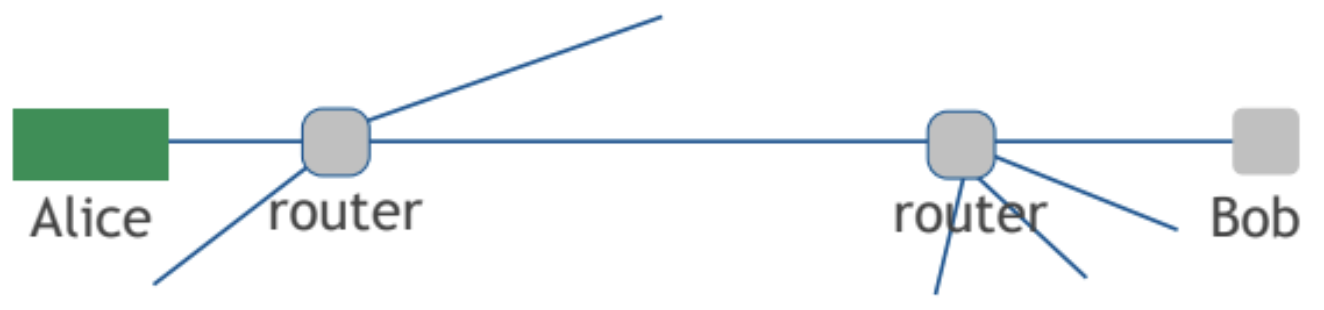
\includegraphics[width=0.6\textwidth]{images/router.png}
\end{center}

These work together to get packets from source to destination.

\subsection{Forwarding: What Each Router Does}
Forwarding is what happens when a packet arrives at a router. The router asks: "Where should I send this packet next?"

This is a quick decision that each router makes for every packet that comes through.

\subsubsection{How Routers Are Set Up}
Each router has several connections (called links). The router gives each link a number, like Link 1, Link 2, Link 3, etc.

The router also has a \textbf{forwarding table} - think of it like a phone book that says "if a packet is going to IP address X, send it out Link Y."

\begin{center}
    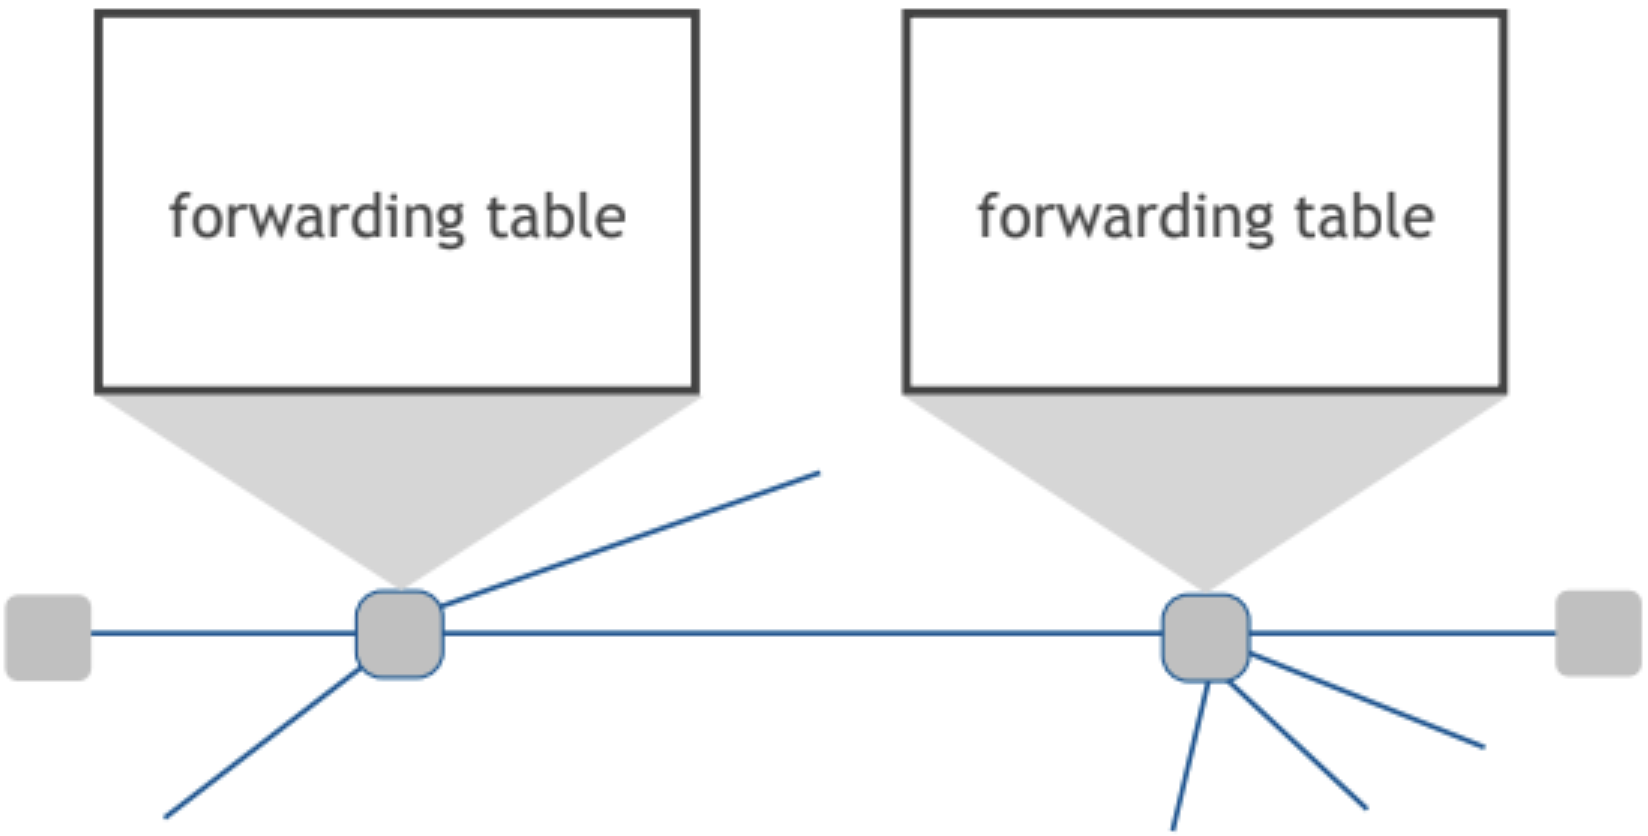
\includegraphics[width=0.6\textwidth]{images/forwarding-table.png}
\end{center}

\subsubsection{Step-by-Step: How Forwarding Works}
Let's say Alice wants to send a packet to Bob, and Bob's IP address is 1.

\begin{center}
    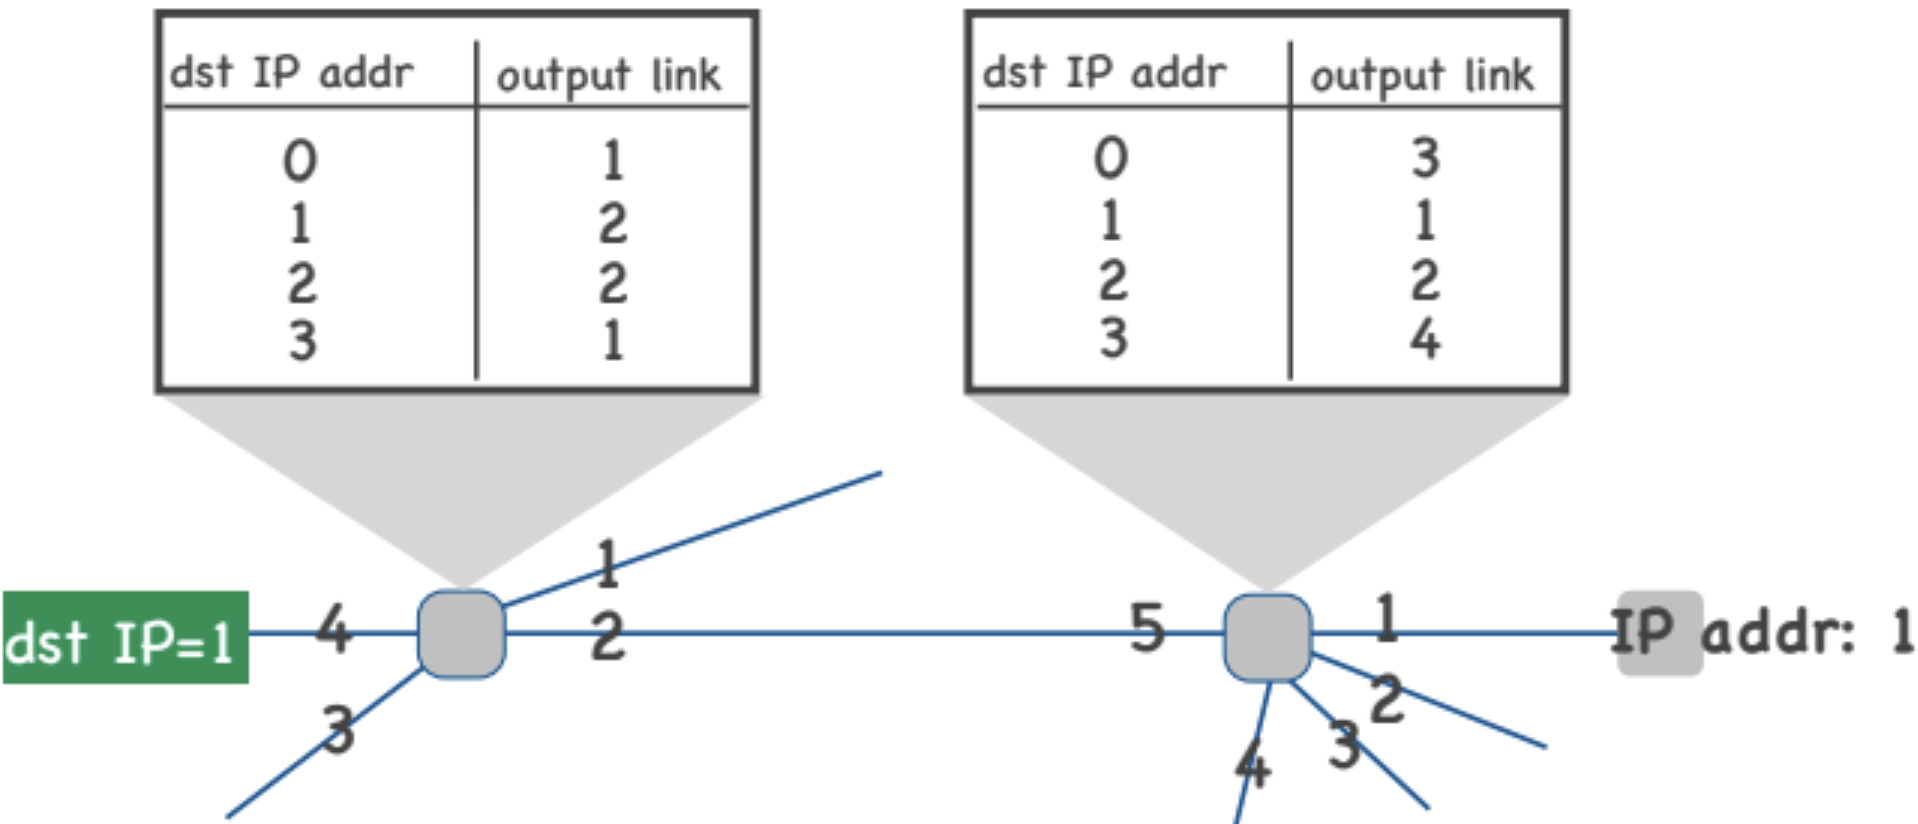
\includegraphics[width=0.6\textwidth]{images/forwarding.png}
\end{center}

Here's what happens:
\begin{enumerate}
    \item Alice puts "1" as the destination IP address in her packet
    \item The first router gets the packet and reads "destination = 1"
    \item The router looks in its forwarding table: "packets for IP 1 go out Link 2"
    \item The router sends the packet out Link 2
    \item The next router does the same thing with its own table
    \item This continues until the packet reaches Bob
\end{enumerate}
\newpage

\subsection{Routing: How Do Forwarding Tables Get Filled?}
Routing is about filling up those forwarding tables. Someone has to tell each router "for IP address X, use Link Y."

\begin{center}
    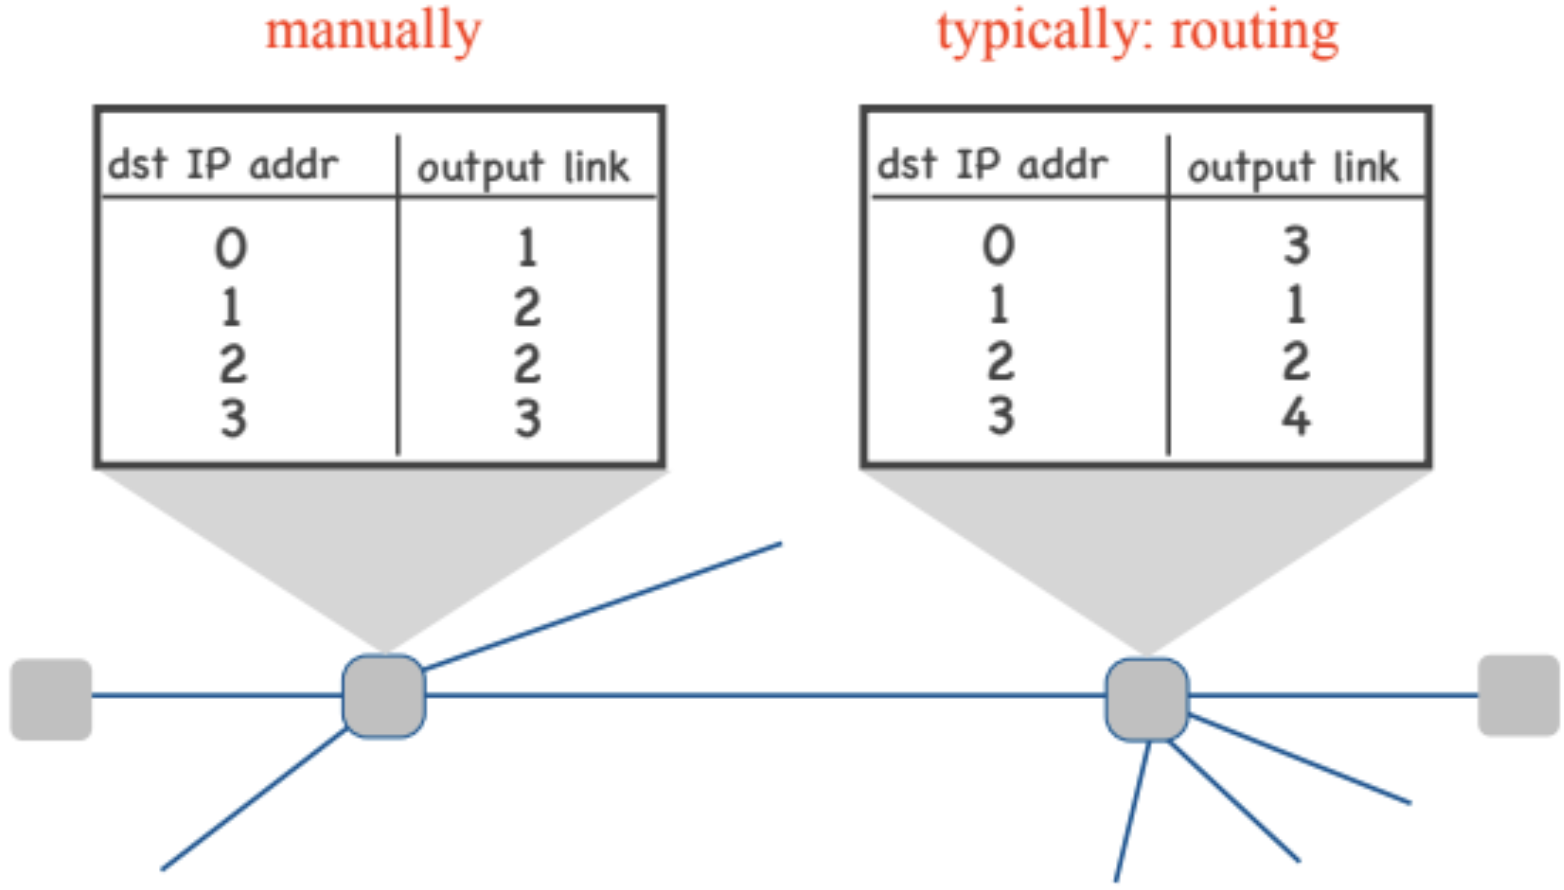
\includegraphics[width=0.6\textwidth]{images/manually-vs-routing.png}
\end{center}

Forwarding asks "where does this packet go?" Routing asks "how do we figure out where packets should go?"

\subsubsection{Two Ways to Fill Forwarding Tables}
\begin{itemize}
    \item \textbf{Manual}: A network administrator types in the rules
    \item \textbf{Automatic}: Software figures it out and fills in the tables
\end{itemize}

Most of the time, it's automatic.

\subsubsection{Centralized Routing: One Brain Controls Everything}
Imagine one smart computer (called a \textbf{network controller}) that knows about all the routers in the network.

\textbf{Good things about this approach:}
\begin{itemize}
    \item The controller sees the whole network, so it can make good decisions
    \item All routers get consistent information
    \item Easy to implement complex policies
\end{itemize}

The controller:
\begin{itemize}
    \item Knows where all routers are and how they connect
    \item Figures out the best forwarding table for each router
    \item Sends this information to each router
\end{itemize}

\subsubsection{Distributed Routing: Routers Talk to Each Other}
Instead of one controller, the routers talk directly to each other and work together to figure out the best routes.

\textbf{Good things about this approach:}
\begin{itemize}
    \item If one router breaks, the others keep working
    \item Works better when you have lots of routers
    \item Routers can quickly adapt to changes nearby
\end{itemize}

\subsubsection{Real Internet: Mix of Both}
The actual Internet uses both approaches in different places.

\section{Making Forwarding Tables Smaller}
Here's a problem: there are about 4 billion possible IP addresses. Do routers really need 4 billion entries in their forwarding tables? 

No! That would be way too big.

\subsection{Using Ranges Instead of Individual Addresses}
Instead of storing every single IP address, routers store \textbf{ranges} of IP addresses.

\begin{center}
    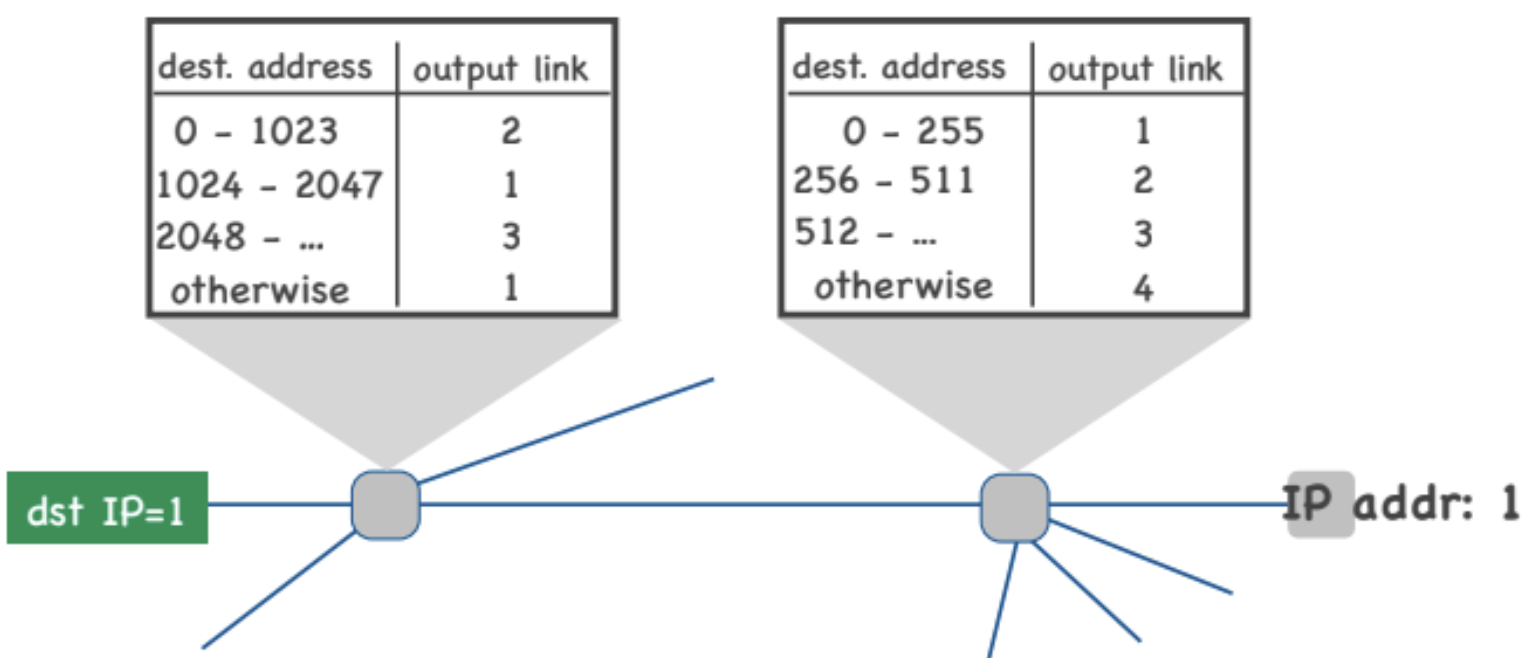
\includegraphics[width=0.6\textwidth]{images/ranges.png}
\end{center}

For example, instead of having separate entries for IP addresses 0, 1, 2, ..., 1023, a router can have one entry that says "all IP addresses from 0 to 1023 go out Link 2."

\subsubsection{How This Works}
When a packet arrives:
\begin{enumerate}
    \item Router looks at the destination IP address
    \item Router finds which range this IP address fits into
    \item Router sends the packet out the link for that range
\end{enumerate}

\begin{center}
    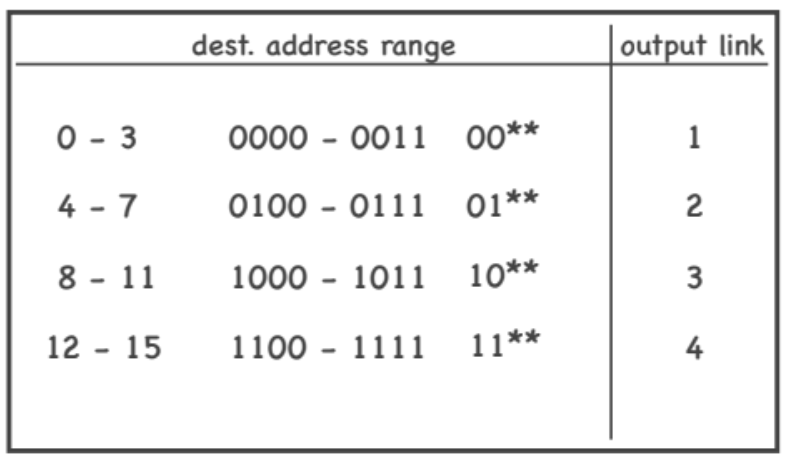
\includegraphics[width=0.6\textwidth]{images/ranges-2.png}
\end{center}

\subsection{IP Prefixes: A Smart Way to Write Ranges}
Let's say we only have 16 IP addresses (0 through 15) to make this easier to understand.

\begin{center}
\begin{tabular}{|c|c|c|c|}
\hline
\textbf{Range} & \textbf{Binary} & \textbf{Prefix} & \textbf{Link} \\
\hline
0-3 & 0000-0011 & 00** & 1 \\
4-7 & 0100-0111 & 01** & 2 \\
8-11 & 1000-1011 & 10** & 3 \\
12-15 & 1100-1111 & 11** & 4 \\
\hline
\end{tabular}
\end{center}

The "00**" means "any address that starts with 00". The ** can be anything (00, 01, 10, or 11).

\subsection{Longest Prefix Matching: Handling Exceptions}
Sometimes we need exceptions. What if most addresses starting with "00" go to Link 1, but address "0011" (which is 3) needs to go somewhere else?

\begin{center}
\begin{tabular}{|c|c|c|}
\hline
\textbf{Prefix} & \textbf{Link} & \textbf{What This Covers} \\
\hline
00** & 1 & addresses 0, 1, 2, 3 \\
0011 & 2 & address 3 (exception!) \\
\hline
\end{tabular}
\end{center}

When a packet for address 3 arrives:
\begin{itemize}
    \item It matches both "00**" and "0011"
    \item The router picks the \textbf{longer} (more specific) match: "0011"
    \item The packet goes to Link 2
\end{itemize}

This is called \textbf{longest prefix matching}.

\subsubsection{More Exceptions = Bigger Tables}
The more exceptions you need, the bigger your forwarding table gets:

\begin{center}
    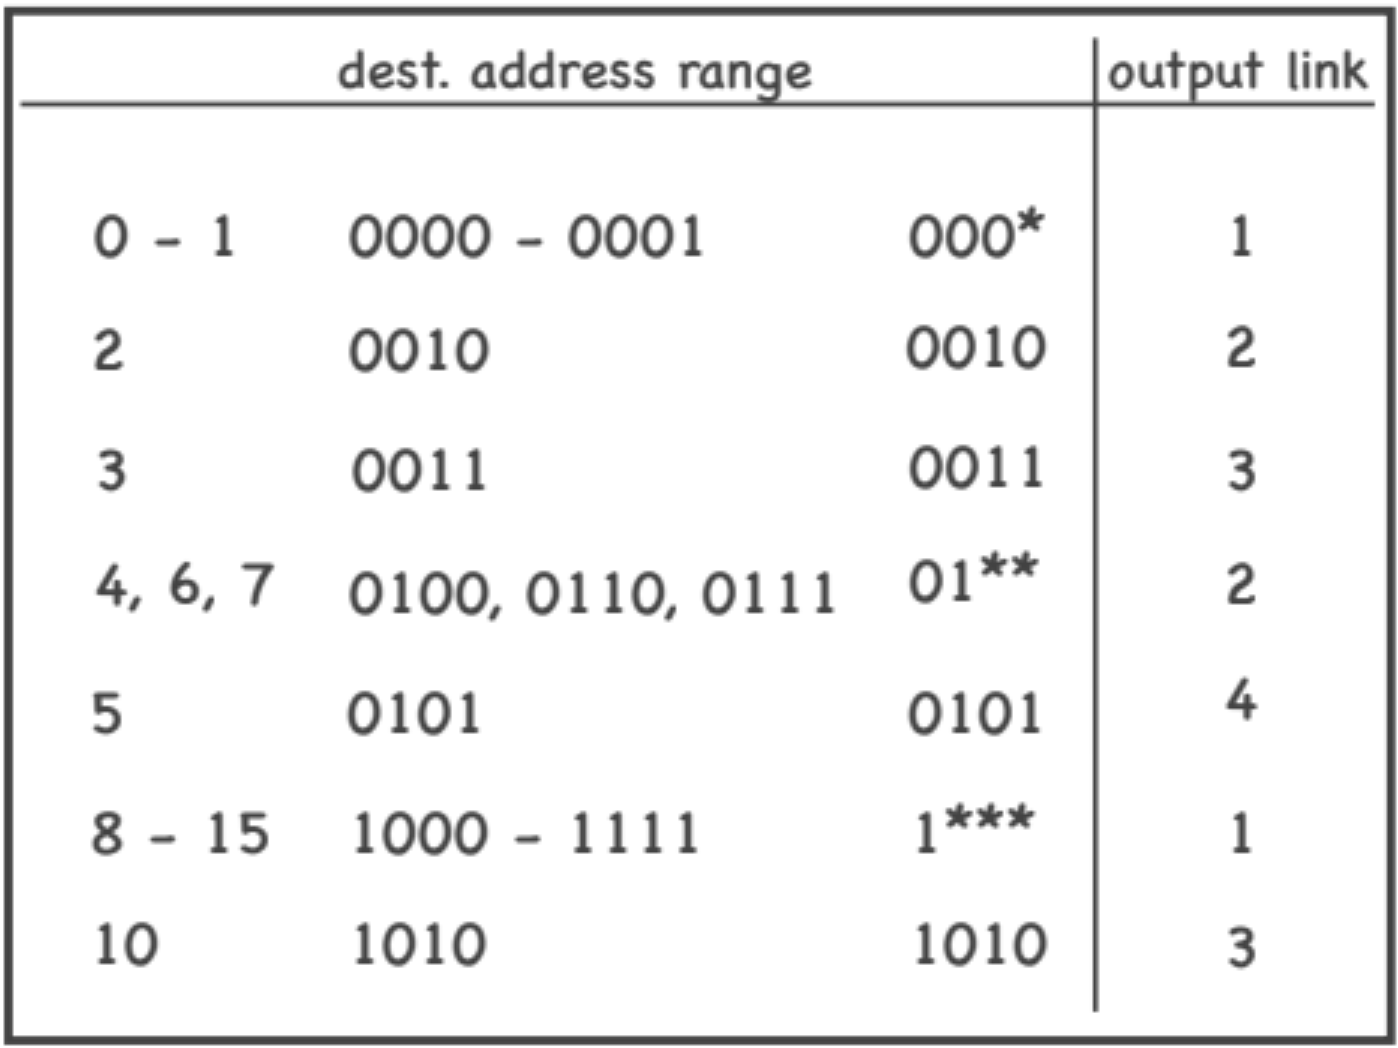
\includegraphics[width=0.45\textwidth]{images/many-exceptions.png}
\end{center}

This is why we want to avoid lots of exceptions.

\section{Why Location Matters for IP Addresses}
For the Internet to work well, IP addresses should be related to location.

\subsection{The Basic Idea}
\begin{itemize}
    \item Devices that are close together should have similar IP addresses
    \item Devices in the same building/city/country should share the same prefix
    \item Similar IP addresses should mean similar locations
\end{itemize}

\subsection{Why This Helps}
\begin{itemize}
    \item \textbf{Smaller forwarding tables}: One entry can cover many destinations
    \item \textbf{Easier routing}: Routes can be grouped together
    \item \textbf{Faster updates}: Changes affect fewer table entries
\end{itemize}

\subsection{What Happens When Location Rules Break}
Here's an example of what goes wrong:

\begin{enumerate}
    \item Let's say all EPFL computers have IP addresses starting with the same prefix
    \item Routers worldwide can have one simple rule: "send all EPFL traffic toward Switzerland"
    \item Now imagine EPFL students travel around the world but keep their EPFL IP addresses
    \item Suddenly routers need special exception rules for each traveling student
    \item If lots of people do this, forwarding tables become huge and unmanageable
\end{enumerate}

This shows why keeping IP addresses tied to location is important for the Internet to work efficiently.

\section{How IP Addresses Are Written}
Now let's learn how to actually write and read IP addresses and IP prefixes.

\subsection{IP Address Format}
An IP address is just a number from 0 to $2^{32}-1$ (that's about 4 billion different numbers).

We could write it in binary (all 0s and 1s), but that would be really long. Instead, we use something called "dot format."

Here's how it works:
\begin{itemize}
    \item Take the 32-bit binary number
    \item Split it into 4 groups of 8 bits each
    \item Convert each group to a regular decimal number (0-255)
    \item Put dots between them
\end{itemize}

\textbf{Example:}
\begin{align}
\text{Binary:} &\quad 11011111\ 00000001\ 00000001\ 00000001 \\
\text{Dot format:} &\quad 223.1.1.1
\end{align}

\subsection{IP Prefix Format}
Remember how we said routers use ranges of IP addresses? We call these ranges \textbf{IP prefixes}.

An IP prefix is written as: \textbf{IP address / mask number}

For example: \texttt{223.1.1.0/24}

\subsubsection{What the Mask Number Means}
The mask number tells us how many bits from the left are "fixed" (can't change).

For \texttt{223.1.1.0/24}:
\begin{itemize}
    \item The first 24 bits must stay the same
    \item The last 8 bits can be anything
    \item This covers all addresses from 223.1.1.0 to 223.1.1.255
\end{itemize}

In binary, this looks like:
\begin{align}
\text{Fixed part:} &\quad 11011111\ 00000001\ 00000001\ ******** \\
\text{Or simply:} &\quad 223.1.1.*
\end{align}

The * means "can be any combination of 0s and 1s."

\subsubsection{Different Ways to Write the Same Prefix}
Here's something interesting: these are all the same IP prefix!
\begin{itemize}
    \item \texttt{223.1.1.0/24}
    \item \texttt{223.1.1.74/24}
    \item \texttt{223.1.1.113/24}
    \item \texttt{223.1.1.*}
\end{itemize}

Why? Because they all have the same first 24 bits. The last 8 bits don't matter for defining the prefix.

\subsubsection{More Examples}
\textbf{Bigger range:} \texttt{223.1.1.0/8}
\begin{itemize}
    \item Only the first 8 bits are fixed
    \item Covers: \texttt{223.*.*.*}
    \item That's all addresses from 223.0.0.0 to 223.255.255.255
\end{itemize}

\textbf{Tricky example:} \texttt{223.1.1.0/12}
\begin{itemize}
    \item First 12 bits are fixed
    \item In binary: \texttt{11011111\ 0000****\ ********\ ********}
    \item Covers: 223.0.0.0 to 223.15.255.255
\end{itemize}

\textbf{Pro tip:} When the mask isn't a multiple of 8 (like /12), it's tricky to figure out the range in your head. It's better to convert to binary and count bits carefully!

\section{How the Internet Is Organized}
The Internet is divided into chunks called \textbf{IP subnets}.

\begin{center}
    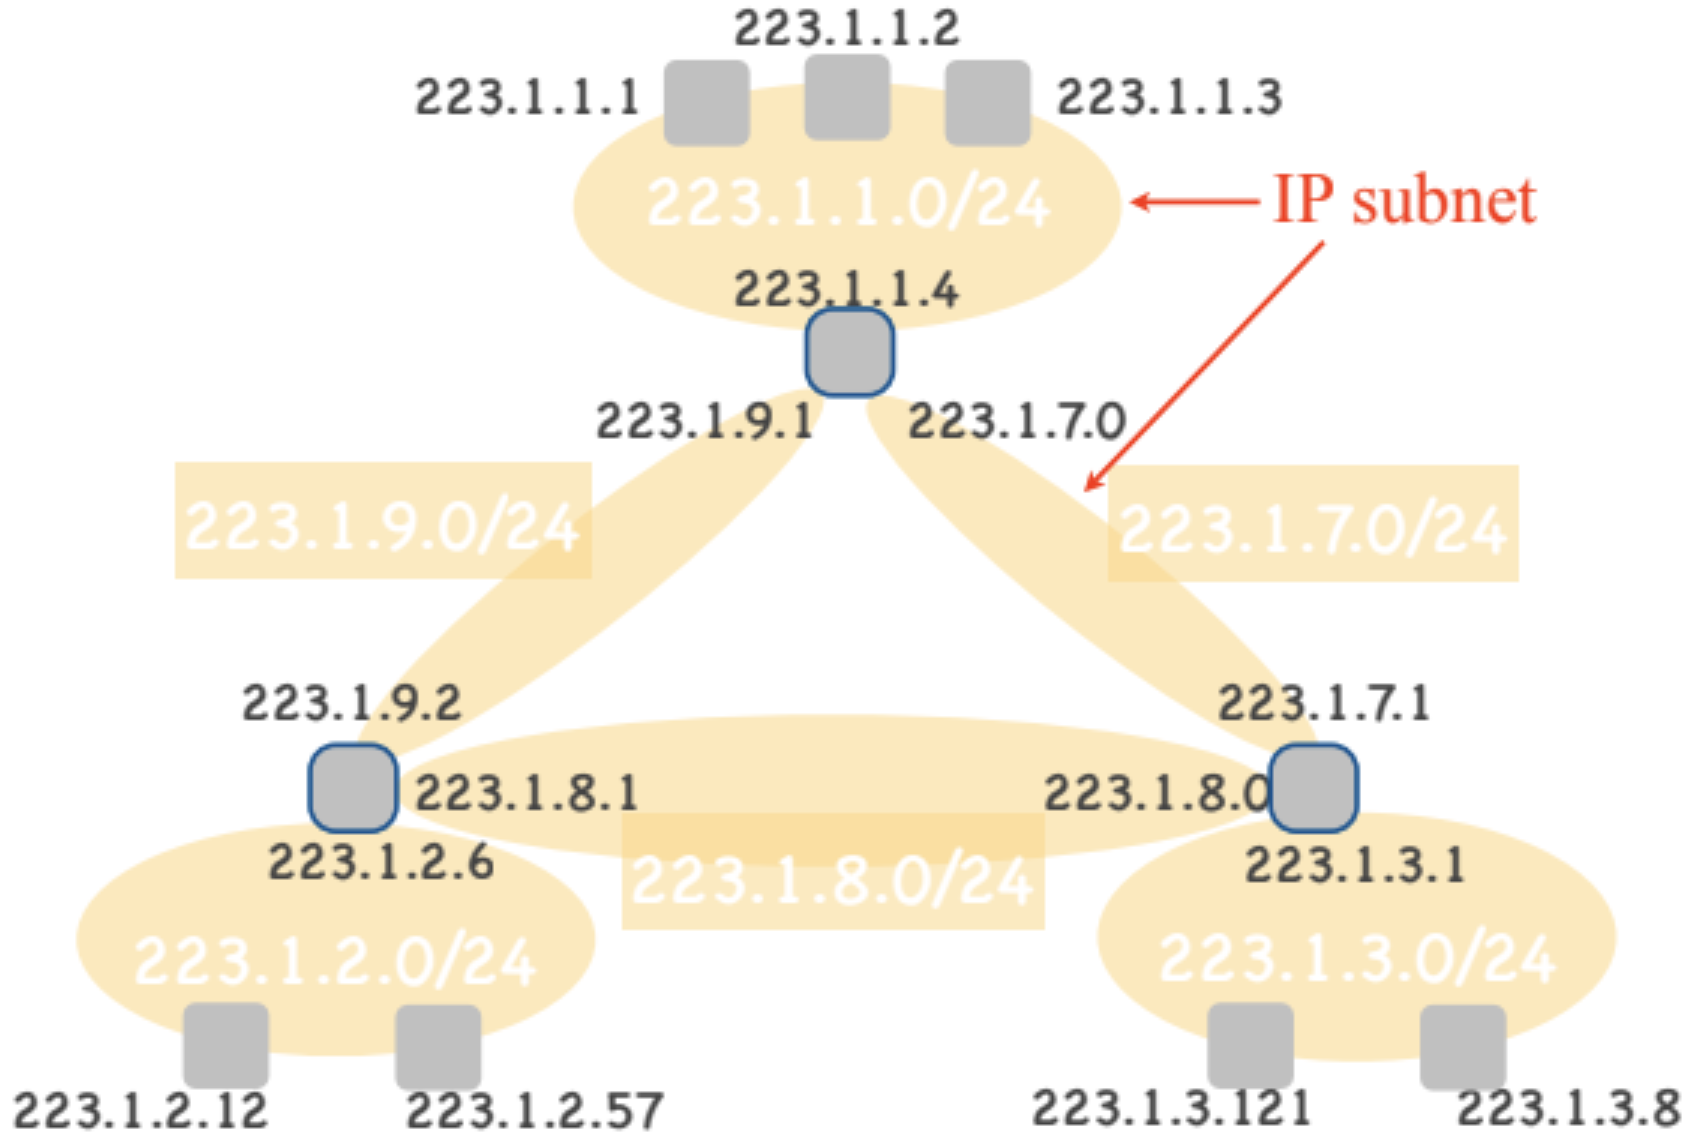
\includegraphics[width=0.6\textwidth]{images/subnets.png}
\end{center}

\subsection{What Is an IP Subnet?}
Think of an IP subnet as a neighborhood:
\begin{itemize}
    \item It contains end-systems (computers, phones, etc.)
    \item It has routers at its "borders" that connect to other neighborhoods
    \item Everyone in the neighborhood has similar addresses (same IP prefix)
    \item The routers don't live "inside" the neighborhood - they're at the edges
\end{itemize}

\subsection{How IP Addresses Are Assigned in Subnets}
Each subnet gets its own IP prefix. For example:
\begin{itemize}
    \item Top subnet might get \texttt{223.1.1.0/24}
    \item Bottom subnet might get \texttt{223.1.2.0/24}
    \item Middle subnets might get \texttt{223.1.3.0/24}, etc.
\end{itemize}

All devices in a subnet get IP addresses from that subnet's prefix.

\subsection{Routers Have Multiple IP Addresses}
Here's something cool: each router has one IP address for each subnet it touches.

Look at the top router in the picture:
\begin{itemize}
    \item It touches 3 different subnets
    \item So it has 3 different IP addresses
    \item Each address belongs to the prefix of that subnet
\end{itemize}

It's like living at the corner of three neighborhoods - you need an address in each one!

\subsection{How Routers Use This Information}
When a router gets a packet, it looks at the destination IP address and asks:
\begin{itemize}
    \item "Is this address in one of my local subnets?" $\rightarrow$ Send it directly there
    \item "Is this address in a foreign subnet?" $\rightarrow$ Forward it toward that subnet
\end{itemize}

For example:
\begin{itemize}
    \item Packet for \texttt{223.1.1.1} $\rightarrow$ "That's in my top subnet!" $\rightarrow$ Send it up
    \item Packet for \texttt{223.1.2.16} $\rightarrow$ "That's in a different subnet" $\rightarrow$ Forward it toward that subnet
\end{itemize}

\section{Special IP Addresses}
\subsection{Broadcast Address}
Each subnet has a special \textbf{broadcast address}:
\begin{itemize}
    \item It's the biggest IP address in the subnet
    \item When you send a packet to this address, it goes to \textit{everyone} in the subnet
    \item For subnet \texttt{223.1.1.0/24}, the broadcast address is \texttt{223.1.1.255}
\end{itemize}

It's like shouting "Hey everyone!" in a room.

\section{How Do Organizations Get IP Addresses?}
\subsection{Getting IP Prefixes}
Organizations get their IP prefixes from:
\begin{itemize}
    \item Their Internet Service Provider (ISP)
    \item A regulatory body (for big organizations)
\end{itemize}

\subsection{Assigning Individual IP Addresses}
Once an organization has its prefix, it assigns individual addresses:

\textbf{For router interfaces:}
\begin{itemize}
    \item Usually done manually by network administrators
\end{itemize}

\textbf{For end-systems (computers, phones):}
\begin{itemize}
    \item Can be done manually
    \item More often done automatically using DHCP (Dynamic Host Configuration Protocol)
\end{itemize}

DHCP is like having an automatic address assignment system - when your laptop joins a network, DHCP gives it an available IP address from that network's range.

\newpage

\section{Best-Effort Delivery}
Here's an important thing to understand about the Internet: it provides \textbf{best-effort delivery}.

\subsection{What Best-Effort Means}
\begin{itemize}
    \item The Internet tries its best to deliver your packets
    \item But it makes \textbf{no promises} that they'll actually arrive
    \item Packets might get lost, delayed, or arrive out of order
    \item The network says "I'll do my best, but no guarantees!"
\end{itemize}

\subsection{Why Best-Effort?}
This might sound bad, but it's actually a smart design choice:
\begin{itemize}
    \item Keeps the network simple and fast
    \item Makes it cheaper to build and operate
    \item Applications can add their own reliability on top if they need it
    \item Works well for most uses (web browsing, email, etc.)
\end{itemize}

Think of it like the postal service - they try to deliver your mail, but sometimes letters get lost. For important things, you can pay extra for certified mail (like how applications can add extra reliability).
\newpage

\section{Virtual Circuits: A Different Way to Do Networking}
So far we've talked about how the Internet works today (packet switching with best-effort delivery). But there's another way to build networks called \textbf{virtual circuits}.
\subsection{The Problem with Best-Effort}
Remember how the Internet makes no promises about packet delivery? Sometimes you want guarantees. For example:
\begin{itemize}
    \item Video calls need consistent, fast delivery
    \item Important business applications can't afford lost packets
    \item Some applications need a minimum guaranteed speed
\end{itemize}
\subsection{How Virtual Circuits Work}
Virtual circuits are like making a reservation at a restaurant - you book resources in advance.

Here's how Alice could get a guaranteed 100 Mbps connection to Bob:

\begin{center}
    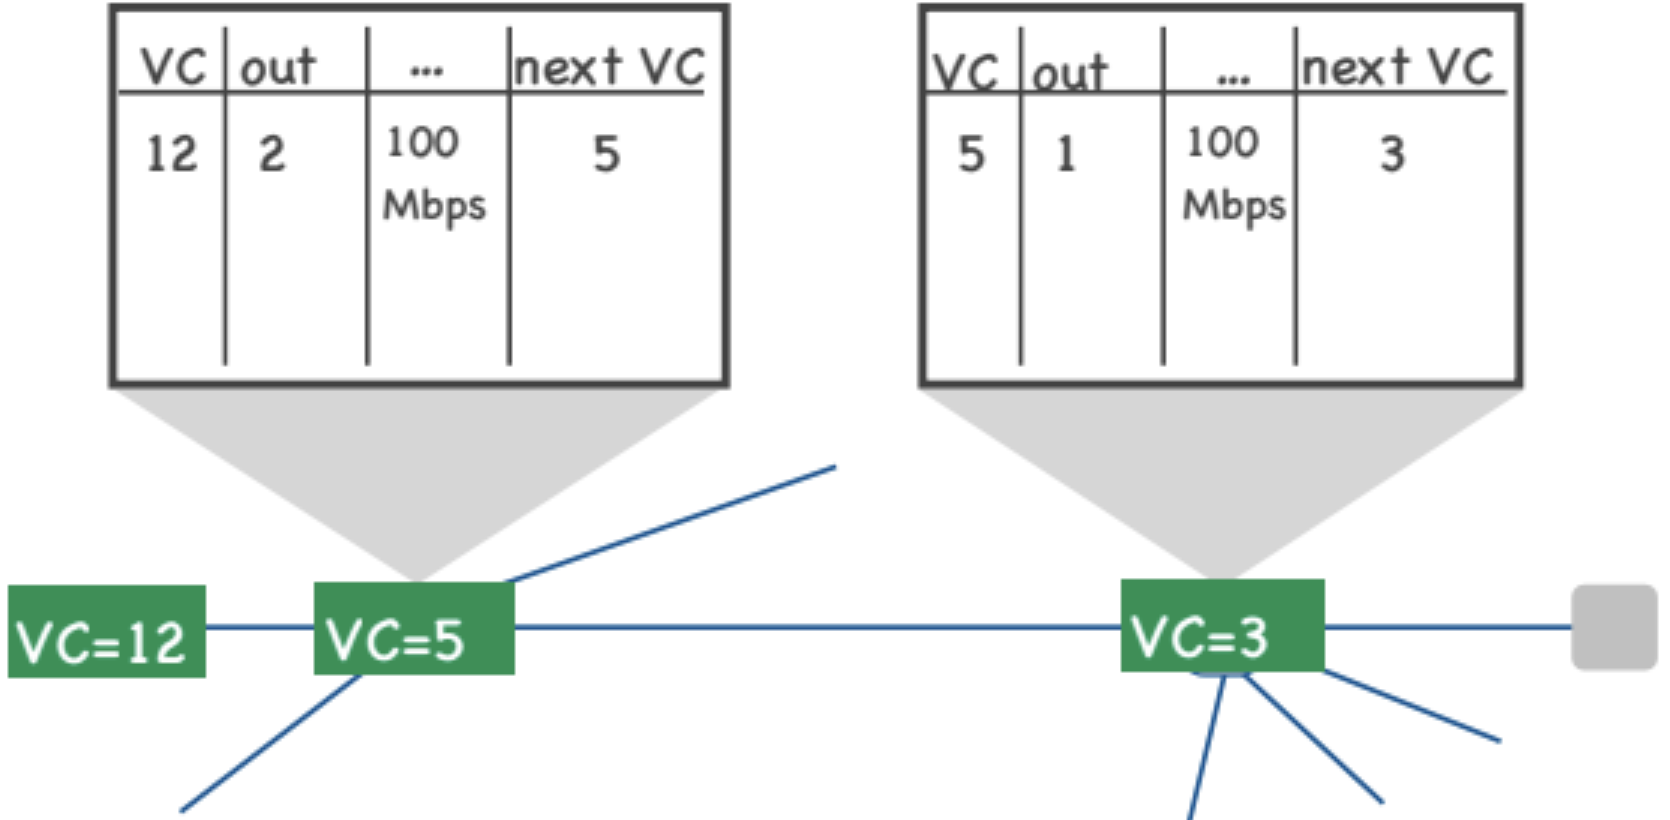
\includegraphics[width=0.6\textwidth]{images/vc.png}
\end{center}

\subsubsection{Step 1: Connection Setup Request}
Alice sends a special "connection-setup request" packet that says: "I want a network connection to Bob with guaranteed 100 Mbps speed."

\subsubsection{Step 2: Each Router Decides}
The packet travels through routers on the path to Bob. Each router asks itself:
\begin{itemize}
    \item "Do I have enough spare capacity to guarantee 100 Mbps?"
    \item "Can I reserve these resources for Alice and Bob?"
\end{itemize}

If a router says yes:
\begin{itemize}
    \item It reserves 100 Mbps of capacity for this connection
    \item It assigns a Virtual Circuit (VC) number to this connection (like giving it a name)
    \item It creates a table entry to remember this reservation
\end{itemize}

For example:
\begin{itemize}
    \item First router assigns VC \#12
    \item Second router assigns VC \#5  
    \item Third router assigns VC \#3
\end{itemize}

\subsubsection{Step 3: Connection Establishment}
If ALL routers on the path agree, Bob gets the request and sends back an "OK" message. This travels back through all the routers so they can coordinate their VC numbers.

Now Alice has a guaranteed 100 Mbps "highway" to Bob!

\subsubsection{Step 4: Using the Virtual Circuit}
When Alice sends packets to Bob:
\begin{itemize}
    \item She puts "VC \#12" in each packet header
    \item First router sees "VC \#12", knows this is Alice's guaranteed connection
    \item Router changes the header to "VC \#5" and forwards to next router
    \item Second router sees "VC \#5", changes to "VC \#3", forwards to third router
    \item And so on until the packet reaches Bob
\end{itemize}

Each router knows exactly how to treat these packets because of the reservation.

\subsection{The Big Challenge: Too Much State}
Here's the problem with virtual circuits: routers have to remember LOTS of information.

\begin{center}
    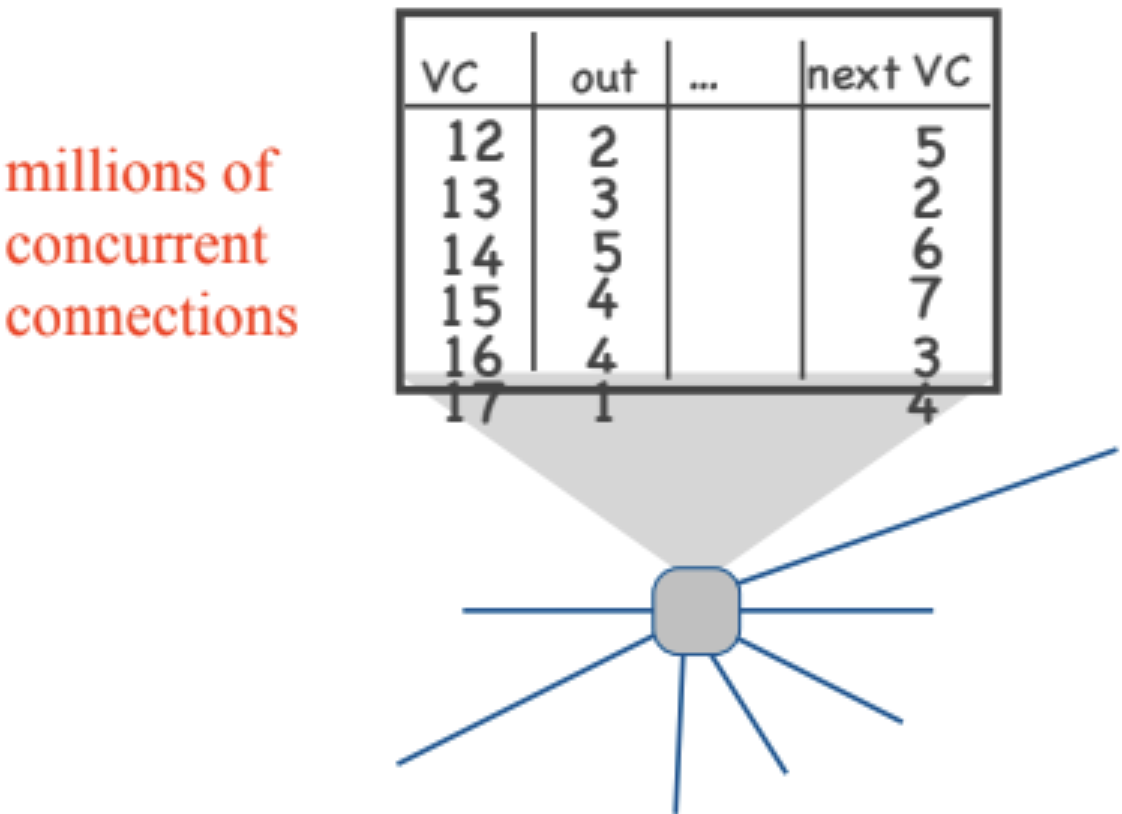
\includegraphics[width=0.45\textwidth]{images/vc-state.png}
\end{center}

\subsubsection{Memory Requirements}
Each router needs to keep a table entry for every active connection passing through it. A busy Internet router might have:
\begin{itemize}
    \item Millions of concurrent connections
    \item Each connection needs memory for state information
    \item This adds up to huge memory requirements
\end{itemize}
\newpage

\subsection{Packet-Switched Networks (Like Today's Internet)}
\textbf{How they work:}
\begin{itemize}
    \item Use packet switching - no network-layer connections
    \item Best-effort delivery (no guarantees)
    \item Routers only store destination prefixes and output links
    \item State is populated by routing protocols
\end{itemize}

\textbf{Good for:} Best-effort service

\subsection{Why the Internet Chose Packet Switching}
Packet switching won because it:
\begin{itemize}
    \item Makes forwarding tables smaller (no per-connection state in routers)
    \item Makes routers simpler (no connection setup/teardown needed)
    \item Eliminates security risks from connection-based attacks
\end{itemize}
\newpage

\section{A Fundamental Internet Principle}
\textit{Every computer should be able to talk to every other computer.}

\subsection{Global Reachability}
The Internet is built on this idea:
\begin{itemize}
    \item Every end-system must be reachable from any other end-system
    \item This requires a globally unique IP address for every end-system
    \item No two devices anywhere in the world should have the same IP address
\end{itemize}

This is like having a postal system where every house has a unique address - no duplicates allowed anywhere!


\section{The IP Address Crisis}
\textit{In the 2000s, we started running out of IP addresses.}

\subsection{The Problem}
\begin{itemize}
    \item IPv4 has about 4 billion possible addresses
    \item The Internet grew faster than expected
    \item We were running out of unique addresses to assign
\end{itemize}

\subsection{Two Solutions}
\textbf{Solution 1: IPv6}
\begin{itemize}
    \item A new version of IP with way more addresses
    \item Deployed in many areas, but not everywhere yet
    \item Long-term solution but takes time to implement
\end{itemize}

\textbf{Solution 2: Network Address Translation (NAT)}
\begin{itemize}
    \item A clever workaround that lets multiple devices share one public IP address
    \item Widely deployed and working today
    \item Has some limitations (which we'll explain)
\end{itemize}

\section{Network Address Translation (NAT)}
\textit{How to let many devices share one public IP address.}

\subsection{The Basic Idea: Private Address Spaces}
Some IP address ranges are designated as "private":
\begin{itemize}
    \item Example: 10.0.0.0/24 is a private range
    \item Multiple networks can use the same private addresses
    \item Like having multiple houses with address "123 Main Street" - it's OK as long as they're in different towns
\end{itemize}

\subsection{The Rule for Private Addresses}
\begin{itemize}
    \item Private IP addresses can only be used within their local network
    \item Packets with private addresses can NEVER leave the local network
    \item It's like calling "John!" in your house - only works if there's only one John there
\end{itemize}

\subsection{How NAT Works: A Step-by-Step Example}
Let's say device 10.0.0.11 (private address) wants to talk to 223.1.1.16 (public address):

\begin{center}
    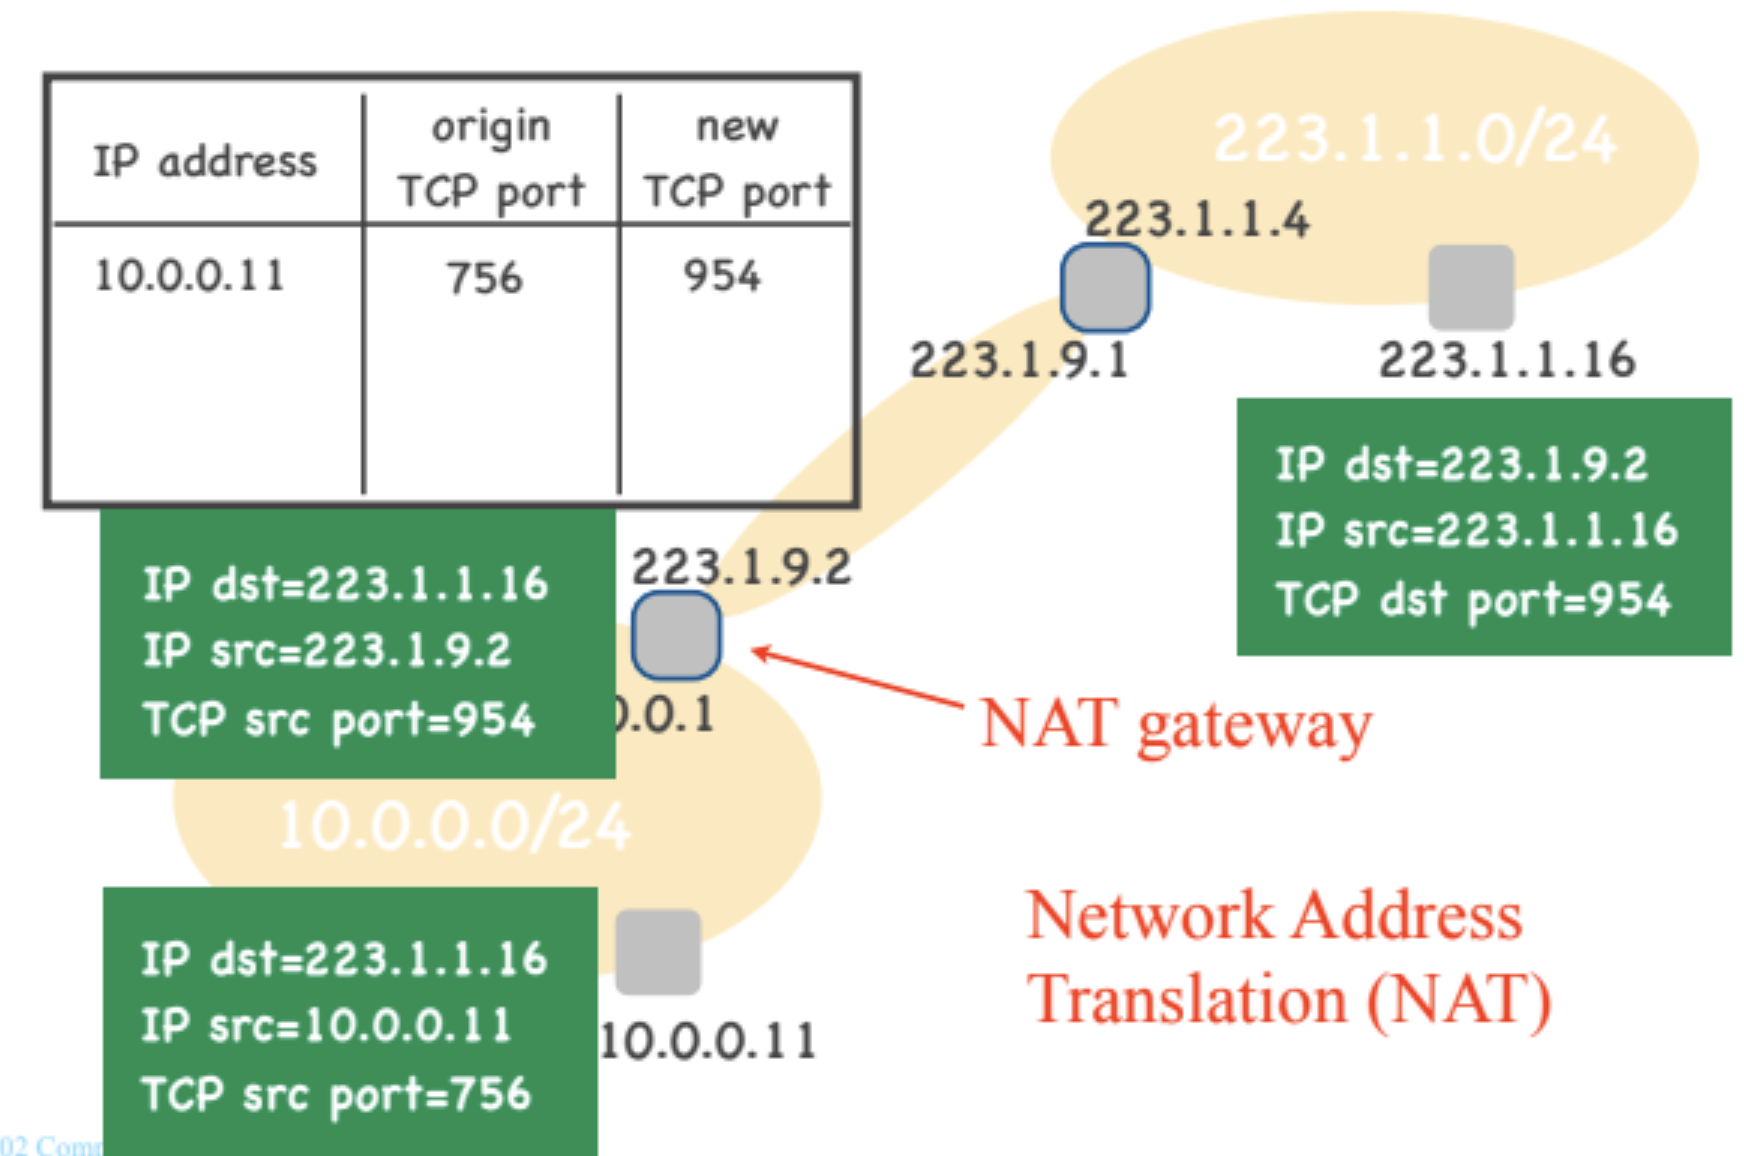
\includegraphics[width=0.6\textwidth]{images/nat.png}
\end{center}

\subsubsection{Step 1: Outgoing Packet}
\begin{itemize}
    \item Device 10.0.0.11 sends packet with source=10.0.0.11, destination=223.1.1.16
    \item It also has a TCP source port (let's say 756)
\end{itemize}

\subsubsection{Step 2: NAT Gateway Translation}
The NAT gateway (border router) does magic:
\begin{itemize}
    \item Replaces source IP 10.0.0.11 with its own public IP 223.1.9.2
    \item Replaces source port 756 with a new port number (say 954)
    \item Remembers this mapping in a table: "10.0.0.11:756 $\leftrightarrow$ 954"
\end{itemize}

\subsubsection{Step 3: Response Packet}
\begin{itemize}
    \item Server 223.1.1.16 responds to 223.1.9.2:954
    \item It thinks it's talking to 223.1.9.2, not 10.0.0.11
\end{itemize}

\subsubsection{Step 4: Return Translation}
\begin{itemize}
    \item NAT gateway gets response packet addressed to 223.1.9.2:954
    \item Looks up port 954 in its table: "Oh, this goes to 10.0.0.11:756"
    \item Changes destination to 10.0.0.11:756 and forwards internally
\end{itemize}

\subsection{What NAT Does}
\textbf{For outgoing packets:}
\begin{itemize}
    \item Rewrites source IP address and port number
    \item Maps original address:port to new port number
    \item Stores this mapping for future use
\end{itemize}

\textbf{For incoming packets:}
\begin{itemize}
    \item Rewrites destination IP address and port number
    \item Uses stored mapping to find the right internal device
\end{itemize}

\section{Problems with NAT}
\textit{NAT works, but it breaks some fundamental Internet principles.}

\subsection{Problem 1: You Can't Reach Devices from Outside}
\begin{itemize}
    \item Devices with private addresses are "hidden" behind the NAT gateway
    \item External devices can't initiate connections to them
    \item Internal devices can call out, but external devices can't call in
    \item Unless you manually configure the NAT gateway with special rules
\end{itemize}

This breaks the global reachability principle!

\subsection{Problem 2: NAT Gateways Need State}
Remember how we said routers shouldn't keep per-connection state? Well, NAT gateways do exactly that:
\begin{itemize}
    \item They remember mappings for every active connection
    \item This is the same problem we had with virtual circuits!
\end{itemize}

\textbf{Why is this OK?}
\begin{itemize}
    \item NAT gateways are usually at the edge (like your home router)
    \item They only handle connections from a small number of devices
    \item Not millions of users like a core Internet router
\end{itemize}

\subsection{Problem 3: It's a Layering Violation}
NAT breaks the clean separation between network layers:
\begin{itemize}
    \item The network layer (IP) shouldn't care about transport layer info (TCP ports)
    \item But NAT has to look at and modify TCP port numbers
    \item This makes the system more complex and fragile
\end{itemize}

\end{document}